% Dòng tiêu đề trang (Running Header)
\noindent
{\fontsize{8.5}{11}\selectfont
\textsf{\textbf{MỤC 2.6}}\hspace{1.5em}\textsf{Giới hạn tại vô cực; Tiệm cận ngang}\hfill\textbf{127}
}
\vspace{3mm}

% Bố cục 2 cột bất đối xứng (Cột lề trái: 38mm, Cột chính: 132mm)
\noindent
\begin{minipage}[t]{38mm}
  % Họa tiết các đường kẻ song song bên trái tiêu đề 2.6
  \vspace*{1.5mm}
  \hfill
  \begin{tikzpicture}
    \foreach \y in {0, 2.5, 5.0, 7.5, 10.0, 12.5} {
      \draw[line width=0.6pt, color=stewartblue!60] (0,\y pt) -- (36pt,\y pt);
    }
  \end{tikzpicture}
  
  % Khoảng cách dóng hàng cho Bảng giá trị
  \vspace{4.2cm}
  \centering
  {\small
  \renewcommand{\arraystretch}{1.15}
  \begin{tabular}{|>{\centering\arraybackslash}p{1.1cm}|>{\centering\arraybackslash}p{1.9cm}|}
  \hline
  $x$ & $f(x)$ \\
  \hline
  $0$ & $-1$ \\
  $\pm 1$ & $0$ \\
  $\pm 2$ & $0.600000$ \\
  $\pm 3$ & $0.800000$ \\
  $\pm 4$ & $0.882353$ \\
  $\pm 5$ & $0.923077$ \\
  $\pm 10$ & $0.980198$ \\
  $\pm 50$ & $0.999200$ \\
  $\pm 100$ & $0.999800$ \\
  $\pm 1000$ & $0.999998$ \\
  \hline
  \end{tabular}
  }
\end{minipage}%
\hfill
\begin{minipage}[t]{134mm}
  % Tiêu đề mục
  \noindent
  {\fontsize{19}{22}\selectfont\bfseries\color{stewartblue} 2.6}\hspace{0.6em}{\fontsize{16}{19}\selectfont\bfseries Giới hạn tại vô cực; Tiệm cận ngang}
  \vspace{0.8em}

  % Đoạn mở đầu
  \noindent
  Trong các Mục 2.2 và 2.4, chúng ta đã nghiên cứu các giới hạn vô cực và tiệm cận đứng của đường cong $y = f(x)$. Ở đó, ta cho $x$ tiến dần đến một số và kết quả là các giá trị của $y$ trở nên lớn tùy ý (dương hoặc âm). Trong mục này, chúng ta cho $x$ trở nên lớn tùy ý (dương hoặc âm) và xem điều gì xảy ra với $y$.
  \vspace{1em}

  % Tiểu mục
  \noindent
  {\color{stewartblue}\rule{1.1ex}{1.1ex}}\hspace{0.5em}{\bfseries Giới hạn tại vô cực và Tiệm cận ngang}
  \vspace{0.5em}

  \noindent
  Hãy bắt đầu bằng việc khảo sát hành vi của hàm số $f$ được xác định bởi
  \[
  f(x) = \frac{x^2 - 1}{x^2 + 1}
  \]
  khi $x$ trở nên lớn. Bảng ở bên trái cho các giá trị của hàm số này chính xác đến sáu chữ số thập phân, và đồ thị của $f$ đã được máy tính vẽ trong Hình 1.
  \vspace{0.3em}

  % Hình 1
  \begin{center}
    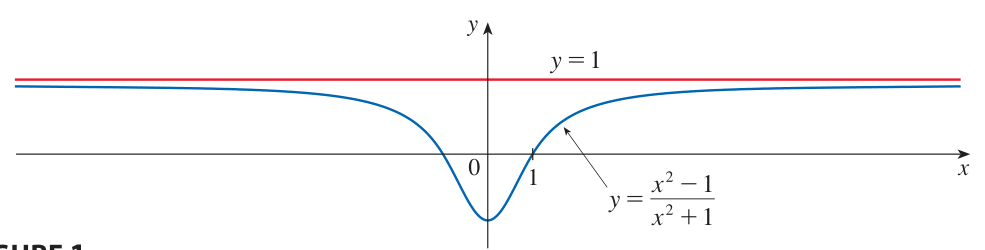
\includegraphics[width=0.88\linewidth]{images/p0162_fig1.png}
  \end{center}
  \vspace{-0.4em}
  \noindent\textbf{HÌNH 1}
  \vspace{0.6em}

  \noindent
  Bạn có thể thấy rằng khi $x$ ngày càng lớn hơn, các giá trị của $f(x)$ ngày càng tiến gần đến $1$. (Đồ thị của $f$ tiến gần đến đường nằm ngang $y = 1$ khi ta nhìn sang bên phải.) Trên thực tế, có vẻ như chúng ta có thể làm cho các giá trị của $f(x)$ gần $1$ tùy ý bằng cách chọn $x$ đủ lớn. Tình huống này được biểu diễn bằng ký hiệu
  \[
  \lim_{x \to \infty} \frac{x^2 - 1}{x^2 + 1} = 1
  \]
  Nói chung, chúng ta sử dụng ký hiệu
  \[
  \lim_{x \to \infty} f(x) = L
  \]
  để chỉ ra rằng các giá trị của $f(x)$ tiến dần đến $L$ khi $x$ ngày càng trở nên lớn hơn.
  \vspace{0.6em}

  % Hộp định nghĩa trực quan
  \begin{tcolorbox}[
    colframe=stewartred,
    colback=white,
    boxrule=0.8pt,
    arc=0pt,
    left=8pt, right=8pt, top=6pt, bottom=7pt
  ]
  \noindent
  \colorbox{stewartred}{\textcolor{white}{\bfseries\fontsize{9}{11}\selectfont\ 1\ }}\hspace{0.5em}{\bfseries\textcolor{stewartred}{Định nghĩa trực quan về Giới hạn tại Vô cực}}\hspace{0.8em}Giả sử $f$ là một hàm số được xác định trên một khoảng $(a, \infty)$ nào đó. Khi đó
  \[
  \lim_{x \to \infty} f(x) = L
  \]
  có nghĩa là các giá trị của $f(x)$ có thể được làm gần với $L$ tùy ý bằng cách yêu cầu $x$ đủ lớn.
  \end{tcolorbox}
  \vspace{0.4em}

  \noindent
  Một ký hiệu khác cho $\lim\limits_{x \to \infty} f(x) = L$ là
  \[
  f(x) \to L \quad \text{khi} \quad x \to \infty
  \]
\end{minipage}

\vfill
% Dòng bản quyền chân trang
\begin{center}
{\fontsize{6.5}{8}\selectfont\color{black!70}
Copyright 2021 Cengage Learning. All Rights Reserved. May not be copied, scanned, or duplicated, in whole or in part. WCN 02-200-203\\[1.5pt]
Editorial review has deemed that any suppressed content does not materially affect the overall learning experience. Cengage Learning reserves the right to remove additional content at any time if subsequent rights restrictions require it.
}
\end{center}
